\section{Versuchsaufbau/-durchführung}
Der wesentliche Aufbau eines Sagnac Interferometers ist in Abbildung \ref{fig:sagnac_interferometer}
dargestellt.
\begin{figure}
\centering
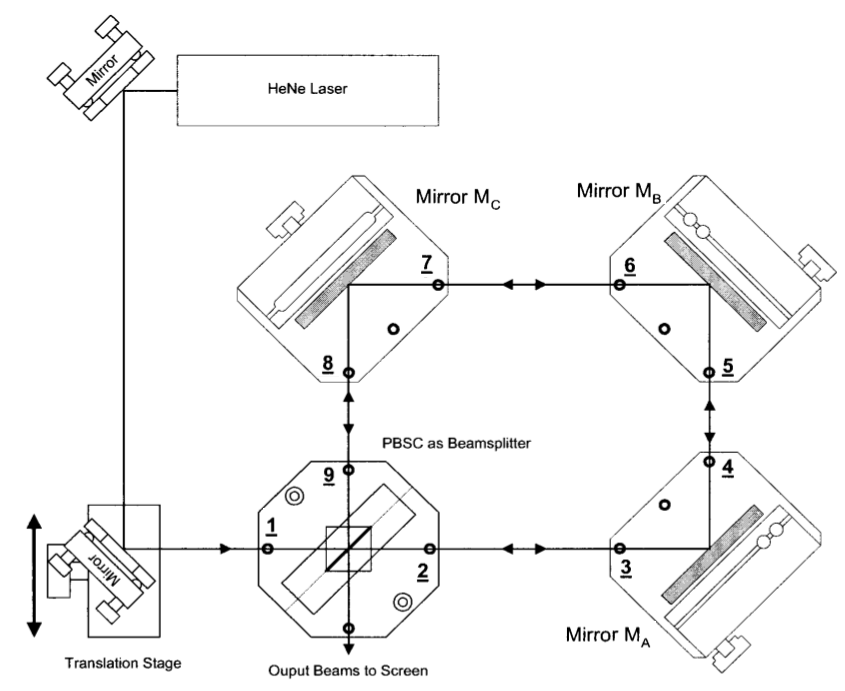
\includegraphics[width=0.6\linewidth]{./content/images/aufbau.png}
\caption{Schmeatischer Aufbau eines Sagnac Interferometers \cite{anleitung64}.}
\label{fig:sagnac_interferometer}
\end{figure}
Als Lichtquelle wird ein $\ce{HeNe}$ Laser mit einer Wellenlänge von
$\lambda\ua{vac}=\SI{632.990}{\nano\meter}$ verwendet. Der Laser wird mittels zweier Steuerspiegel
über einen PBSC in das Interferometer eingeleitet. Ausgekoppelt wird das Licht, wie
in Abbildung \ref{fig:sagnac_interferometer} zu erkennen, über die vierte Seite
des Würfels.
Der Ausgangstrahl wird zur Bestimmung des Brechungsindexes in ein weiteren
PBSC geleitet, der jedoch um $\SI{45}{\degree}$ in der Horizontalen gedreht ist.
Die Drehung des PBSC hat dieselbe Auswirkung auf die Polarisation, wie ein Polarisationsfilter mit
einem Filterwinkel von $\SI{45}{\degree}$. Hierdurch wird das zunächst senkrecht
polarisierte Licht (vgl. Abb. \ref{fig:pbsc}) auf die Filterachse projiziert und
ist somit interferenzfähig. Im Gegensatz zu einem Polarisationsfilter, erhält ein
PBSC näherungsweise die Eingangsleistung.
Das von dem zweiten PBSC aufgeteilte Licht wird
anschließend auf zwei Photodioden gerichtet.

\subsection{Justage}
Zu Beginn wird der Versuchsaufbau in einigen Schritten justiert werden.
Erklärt wird die Justage mit den in Abbildung \ref{fig:sagnac_interferometer} verwendeten Bezeichnern.
Nachdem die benötigten Komponenten auf dem optischen Tisch montiert sind,
wird mit Hilfe von zwei Justagehilfen, der Lichtstrahl optimal auf den Spiegel $M_C$
ausgerichtet. Hierbei wird der von $M_A$ kommende Strahl blockiert.
Anschließend werden die Justagehilfen dazu verwendet, um den Laserstrahl optimal auf
die Spiegel $M_A$ und $M_B$ auszurichten. Vor dem ersten PCBS wird zusätzlich noch ein Polarisationsfilter
mit einem Filterwinkel von $\SI{45}{\degree}$ platziert. Zusätzlich werden mit Hilfe der Justagehilfen
und des zweiten Steuerspiegels die beiden senkrecht zueinander polarisierten Strahlen räumlich (horizontal)
voneinander getrennt.

Nachdem das Interferometer ausgerichtet ist, können die beiden Lichtstrahlen an der vierten Seite des PCBS
, mit einem Schirm, untersucht werden.
Liegen die beiden Lichtpunkte, auf dem Schirm, nicht aufeinander, werden mit Hilfe der
Feinschrauben der Spiegel $M_A$, $M_B$ und $M_C$ eine Nachjustage vorgenommen. Wichtig ist, dass zum
jetzigen Zeitpunkt noch keine Interferenzen beobachtet werden können. Erst nach
dem Einbau eines weiteren Polarisationsfilter (Filterwinkel $\SI{45}{\degree}$)
ist es möglich Interferenzen auf dem Schirm zu erkennen.
Das Interferenzbild soll so eingestellt werden, dass die
"Interferenzfrequenz" null ist, dazu können die Feinschrauben der Spiegel
$M_A$ und $M_C$ verwendet werden.

Wurde die "Interferenzfrequenz" minimiert, wird der zweite Polarisationsfilter wieder
entfernt und stattdessen der um $\SI{45}{\degree}$ geneigte PBSC mit den Photodioden
montiert. Mit "Interferenzfrequenz" ist die Anzahl der Streifen des Interferenzmusters
gemeint, die bei der Überlagerung der beiden Strahlen entstehen.
Bevor nun die Brechungsindizes von Luft und Glas bestimmt werden, wird eine
Kontrastbestimmung durchgeführt. Hierzu mehr im nächsten Kapitel.

\subsection{Kontrastbestimmung}\label{sec:Kontrastbestimmung}
Der Kontrast des Interferometers ist ein Maß für das Auflösungsvermögen und wird
wie folgt definiert
\begin{equation}
  \label{eq:kontrast}
  K = \frac{I\ua{max} - I\ua{min}}{I\ua{max}+I\ua{min}}.
\end{equation}
Für die Bestimmung der Intensitäten $I\ua{max}$ und $I\ua{min}$ wird der zweite
PBSC und die Glasprobe benötigt. Die Probe
besteht aus zwei Gläsern die jeweils zu einem der räumlich separierten Strahlen
des Interferometers einen Winkel von $\SI{10}{\degree}$ stehen. Durch die Gläser wird
ein Gangunterschied bzw. eine Phasendifferenz zwischen den beiden Strahlen erzeugt.
Hierzu kann die Probe um $\SI{10}{\degree}$ gedreht werden. Zu beachten ist, dass
bei einer Beispielweisen Drehung der Gläser um $\SI{1}{\degree}$, ein Glas
einen Winkel von $\SI{9}{\degree}$ und das Andere von $\SI{11}{\degree}$ zu den jeweiligen
Strahlen besitzen. Somit ist die Gesamtwinkeländerung in Gleichung \eqref{eq:entwicklung_interferenzmaxima} $\theta = \SI{2}{\degree}$.
Die Intensität wird nun mit Hilfe einer Photodiode und einem Oszilloskop
gemessen. Die Messungen erfolgen bei verschiedenen Filterwinkeln des Polarisationsfilters.
Die Projektion des der Polarisation des elektrischen Feldes $\vec{E_0}=E\ua{0,x}\vec{e}\ua{x}
+E\ua{0,y}\vec{e}\ua{y}$, kann mathemaisch wie folgt beschrieben werden:
\begin{equation}
  \label{eq:projektion_des_e_feldes}
  \vec{E_0}'=\left(E\ua{0,x}\vec{e}\ua{x}+E\ua{0,y}\vec{e}\ua{y}\right) \begin{pmatrix} \cos(\vartheta) \\ \sin(\vartheta) \end{pmatrix}
\end{equation}
Wird die Gleichung \eqref{eq:projektion_des_e_feldes} in Formel \eqref{eq:Interferenz_enstehung}
eingesetzt so ergibt sich
\begin{equation}
  \label{eq:Interferenz}
  I\propto E^2(1+2\cos(\vartheta)\sin(\vartheta)\cos(\Delta\phi)).
\end{equation}
Nachdem das elektrische Feld den zweiten PBSC durchquert, besitzen die beiden elektrischen Felder
dieselbe Polarisation, $\delta = 0$. Aus der Gleichung \eqref{eq:Interferenz}
kann $I\ua{max}$ und $I\ua{min}$ abgeleitet werden:
\begin{align}
  \label{eq:I_max_und_I_min}
  \begin{aligned}
  I\ua{max} & = E^2(1+2\cos(\vartheta)\sin(\vartheta)), \quad \text{Konstruktive Interferenz} \\
  I\ua{min} & = E^2(1-2\cos(\vartheta)\sin(\vartheta)), \quad \text{Destuktive Interfetenz}.
\end{aligned}
\end{align}
Werden nun die Gleichungen \eqref{eq:I_max_und_I_min} in die Definition des Kontrastes \eqref{eq:kontrast}
eingesetzt, ergibt sich die Winkelabhängigkeit des Kontrastes
\begin{equation}
  \label{eq:first_definition_kontrast}
  K=\sin(2\vartheta).
\end{equation}
Der Wert des Kontrastes sollte immer größer gleich null sein, deshalb wird Gleichung \eqref{eq:first_definition_kontrast},
wie folgt umdefiniert
\begin{equation}
  \label{eq:definition_dontrast}
  K:=\be{\sin(2\vartheta)}.
\end{equation}
Der Polarisationsfilter wird für die nachfolgende Bestimmung der Brechungsindizeis
so eingestellt, dass der Kontrast maximal ist.
\subsection{Bestimmung der Brechungsindizes}
Untersucht wird der Brechungsindex von Luft und von Glas.
Für die Luftbestimmung wird eine Gaszelle der Länge $L=\SI{100\pm0.1}{\milli\meter}$
verwendet. Evakuiert wird die Zelle mit Hilfe einer Vakuumpumpe auf einen
Druck in der Größenordnung von $p\sim\mathcal{O}(\SI{10}{\milli\bar})$.
Die Anzahl der Interferenzmaxima wird mit zwei Photodioden bestimmt.
Hierfür werden die Signale der Dioden subtrahiert, um so unabhängiger gegenüber
Leistungsfluktuationen des Lasers zu sein. Jeder Nulldurchgang der Subtraktion
repräsentiert ein Interferenzmaximum. Die Nulldurchgänge werden mit einem digitalen
Zählwerk gezählt. Nach der Evakuierung der Gaszelle wird langsam Luft in die Zelle
gelassen und in $\SI{100}{\milli\bar}$ Schritten die gezählten Maxima notiert. Die Prozedur wird
drei Mal durchgeführt.

Der Brechungsindex von Glas wird mit der in Abschnitt \ref{sec:Kontrastbestimmung}
beschriebenen Glasprobe bestimmt. Die Gläser besitzen eine Dicke von $H=\SI{1.0}{\milli\meter}$.
Hierfür werden, wie bei der Gasuntersuchung,
die beiden Signale der Photodioden subtrahiert. Die Anzahl der Maxima
werden in Abhängigkeit des Drehwinkels aufgenommen.
Der Festkörper wird zehn Mal um
$\SI{10}{\degree}$ gedreht. Nach jeder Drehung wird das Zählwerk zurückgesetzt.
